\documentclass[tikz, border=2pt]{standalone}

\usepackage{helvet}
\renewcommand{\familydefault}{\sfdefault}

\usepackage[EULERGREEK]{sansmath}
\sansmath
\usetikzlibrary{arrows.meta}

\begin{document}%

\begin{tikzpicture}[line width=2pt]
\tikzset{>={Latex[width=3mm,length=4mm]}}

% % grid
% \draw[help lines] (-5, -5) grid (13, 18);

\definecolor{gold}{RGB}{255,215,3}

\definecolor{darkblue}{RGB}{2,0,139}

\node[inner sep=0pt] (figa) at (0,5)
{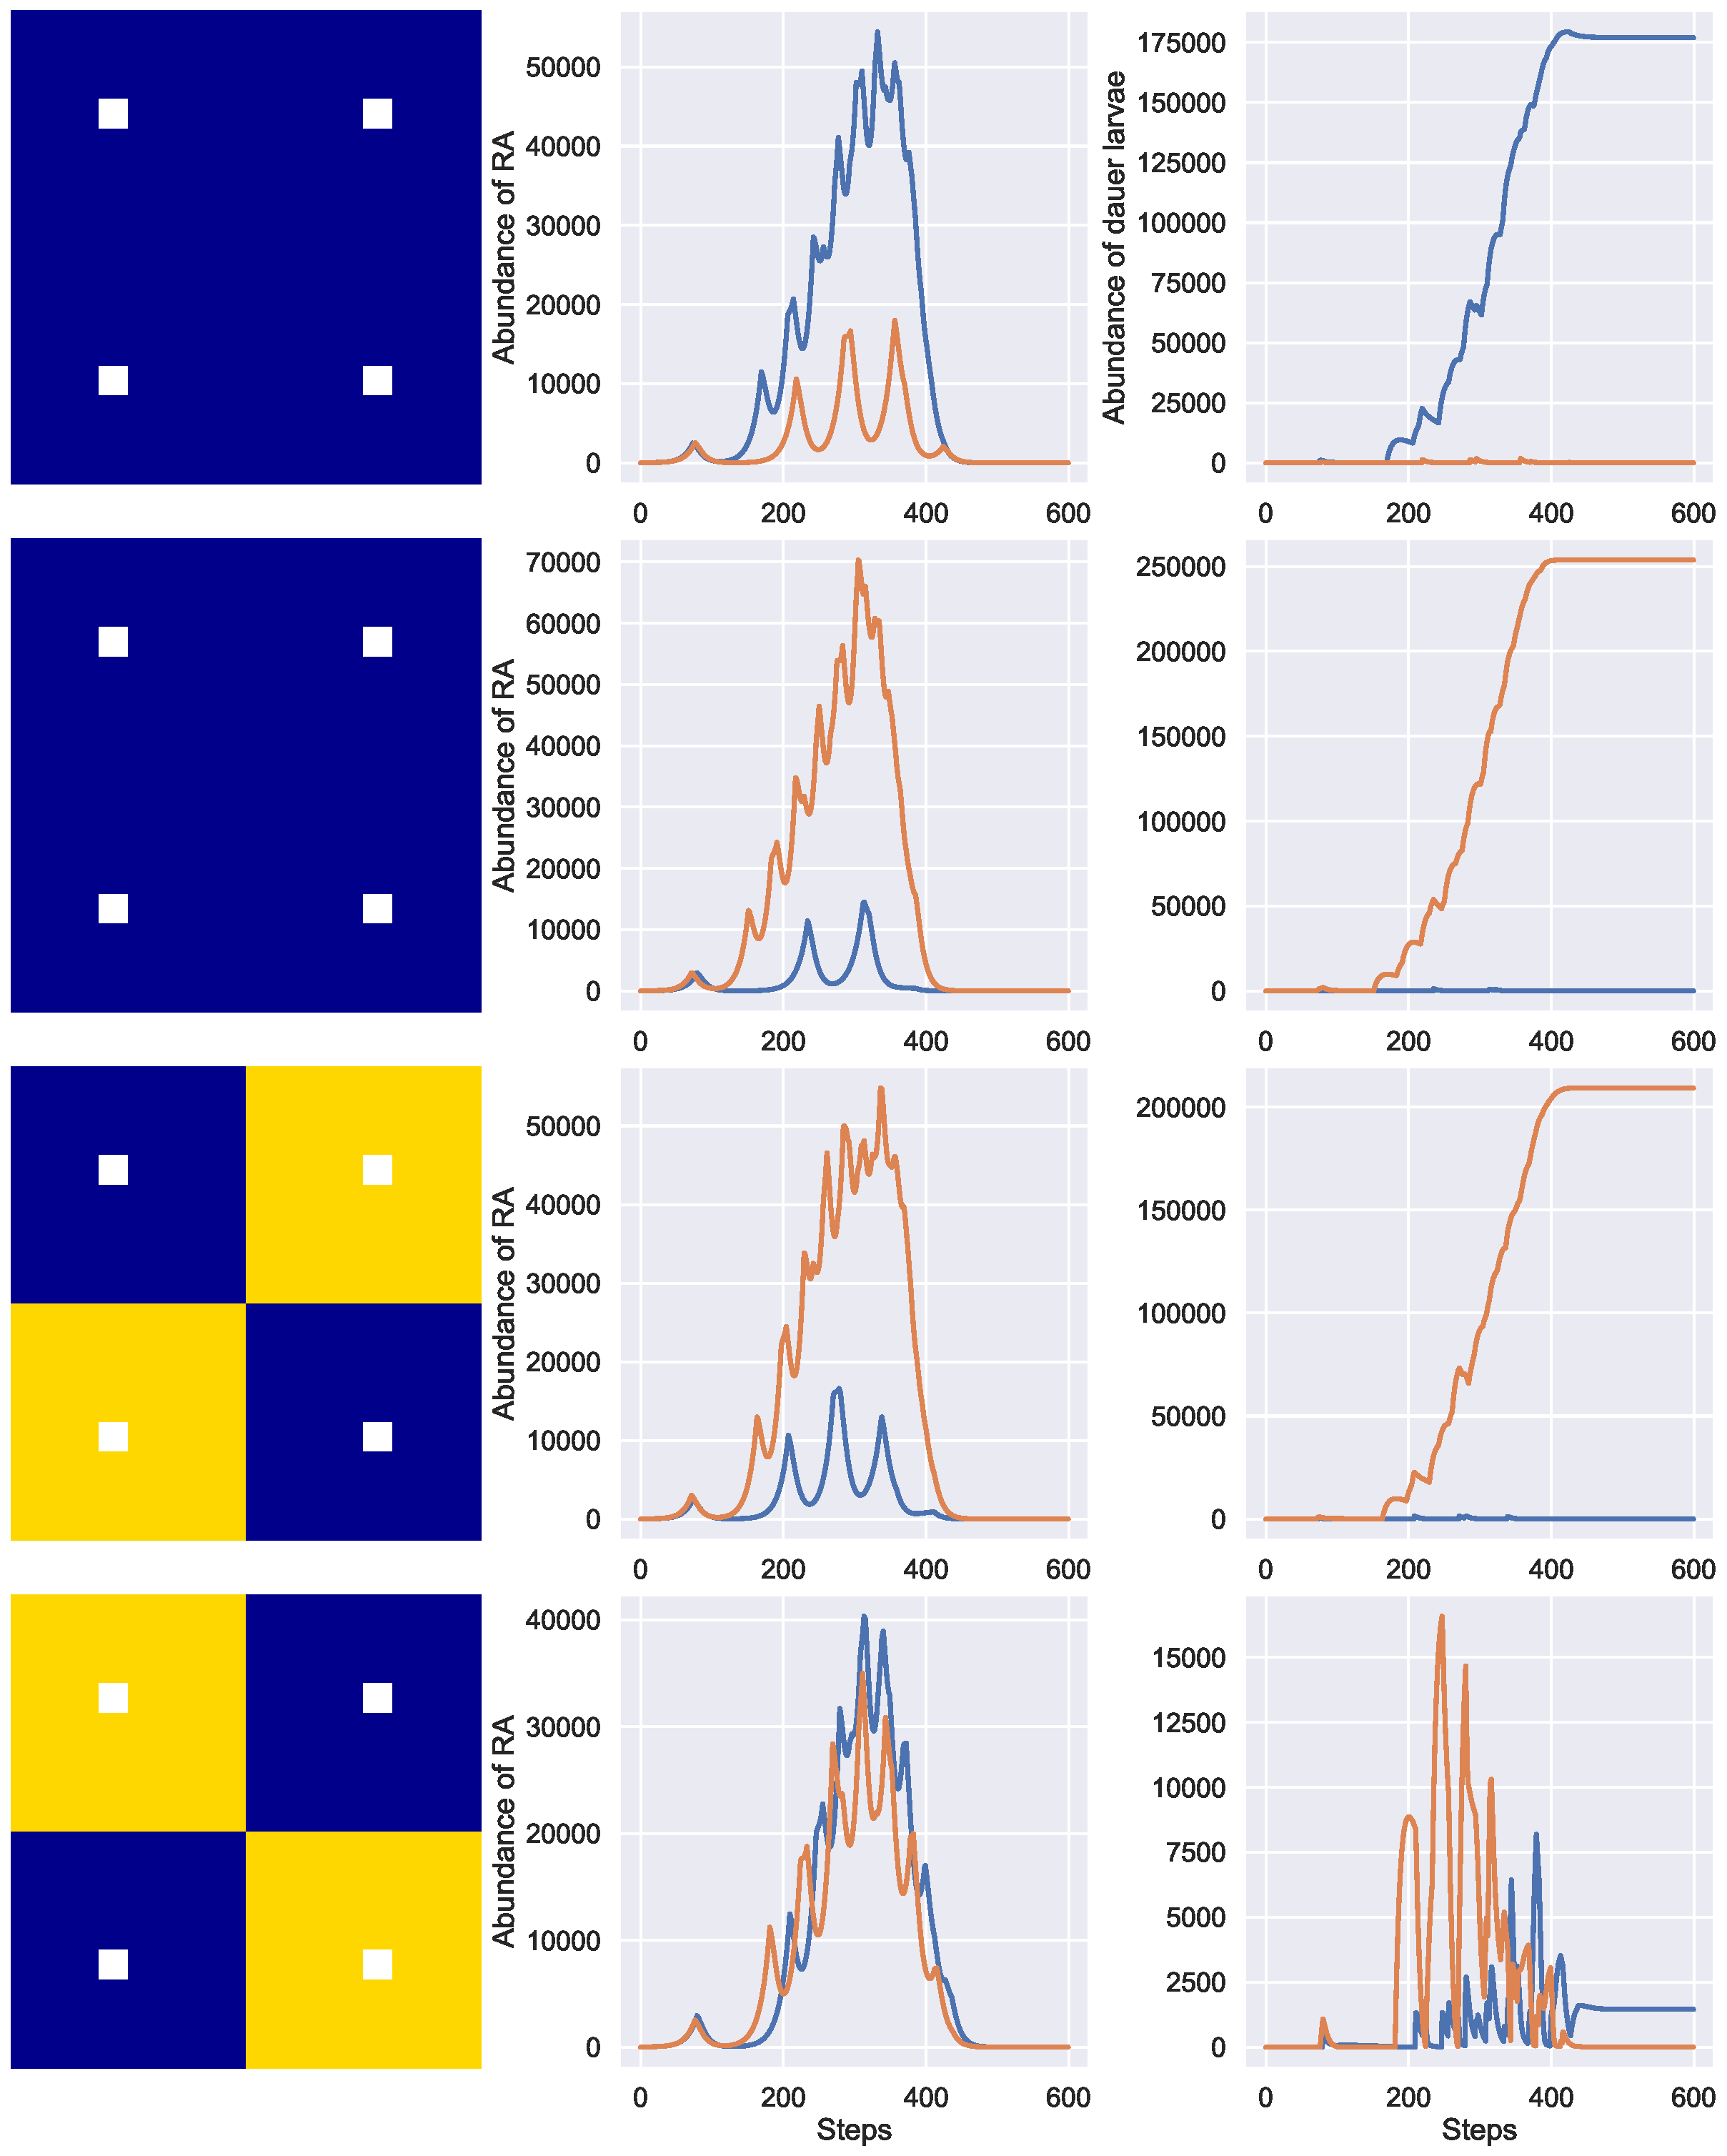
\includegraphics[width=.8\textwidth]{../torus_patt_non_rand.pdf}};

\node[inner sep=0pt] (figa) at (10,5)
{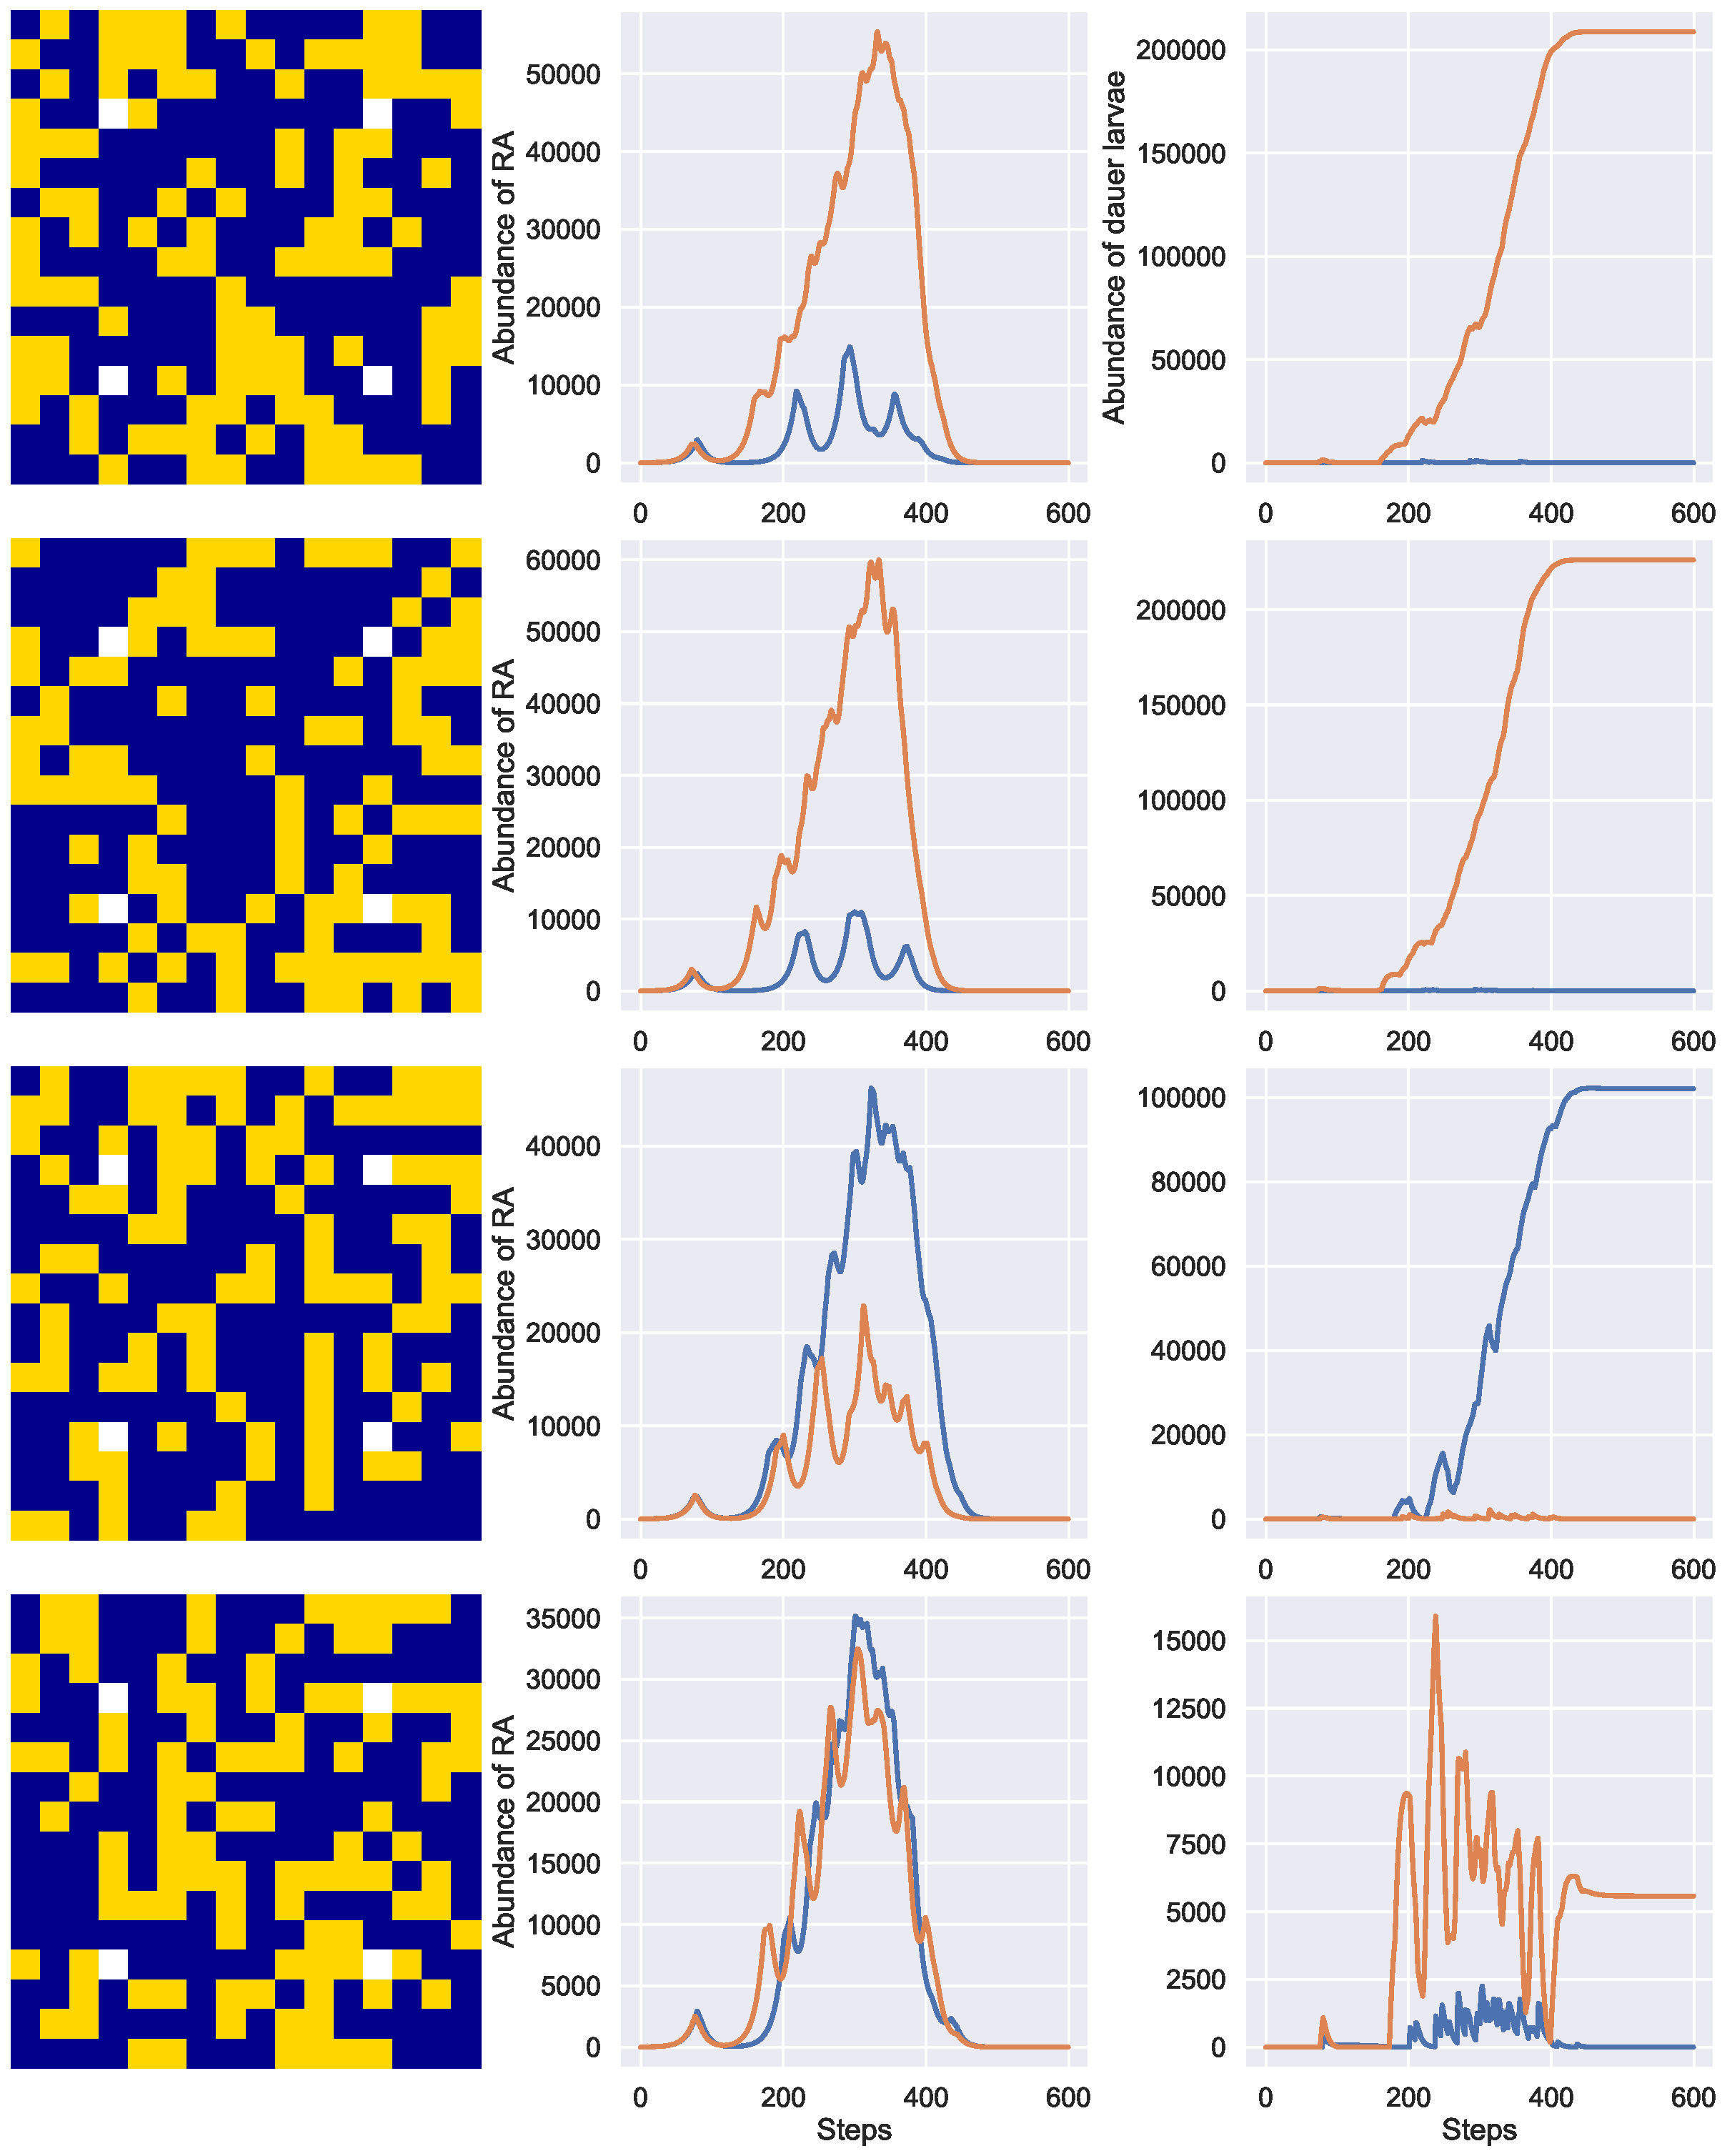
\includegraphics[width=0.8\textwidth]{../torus_patt.pdf}};



\node[inner sep=0pt] (figa) at (5.,13)
{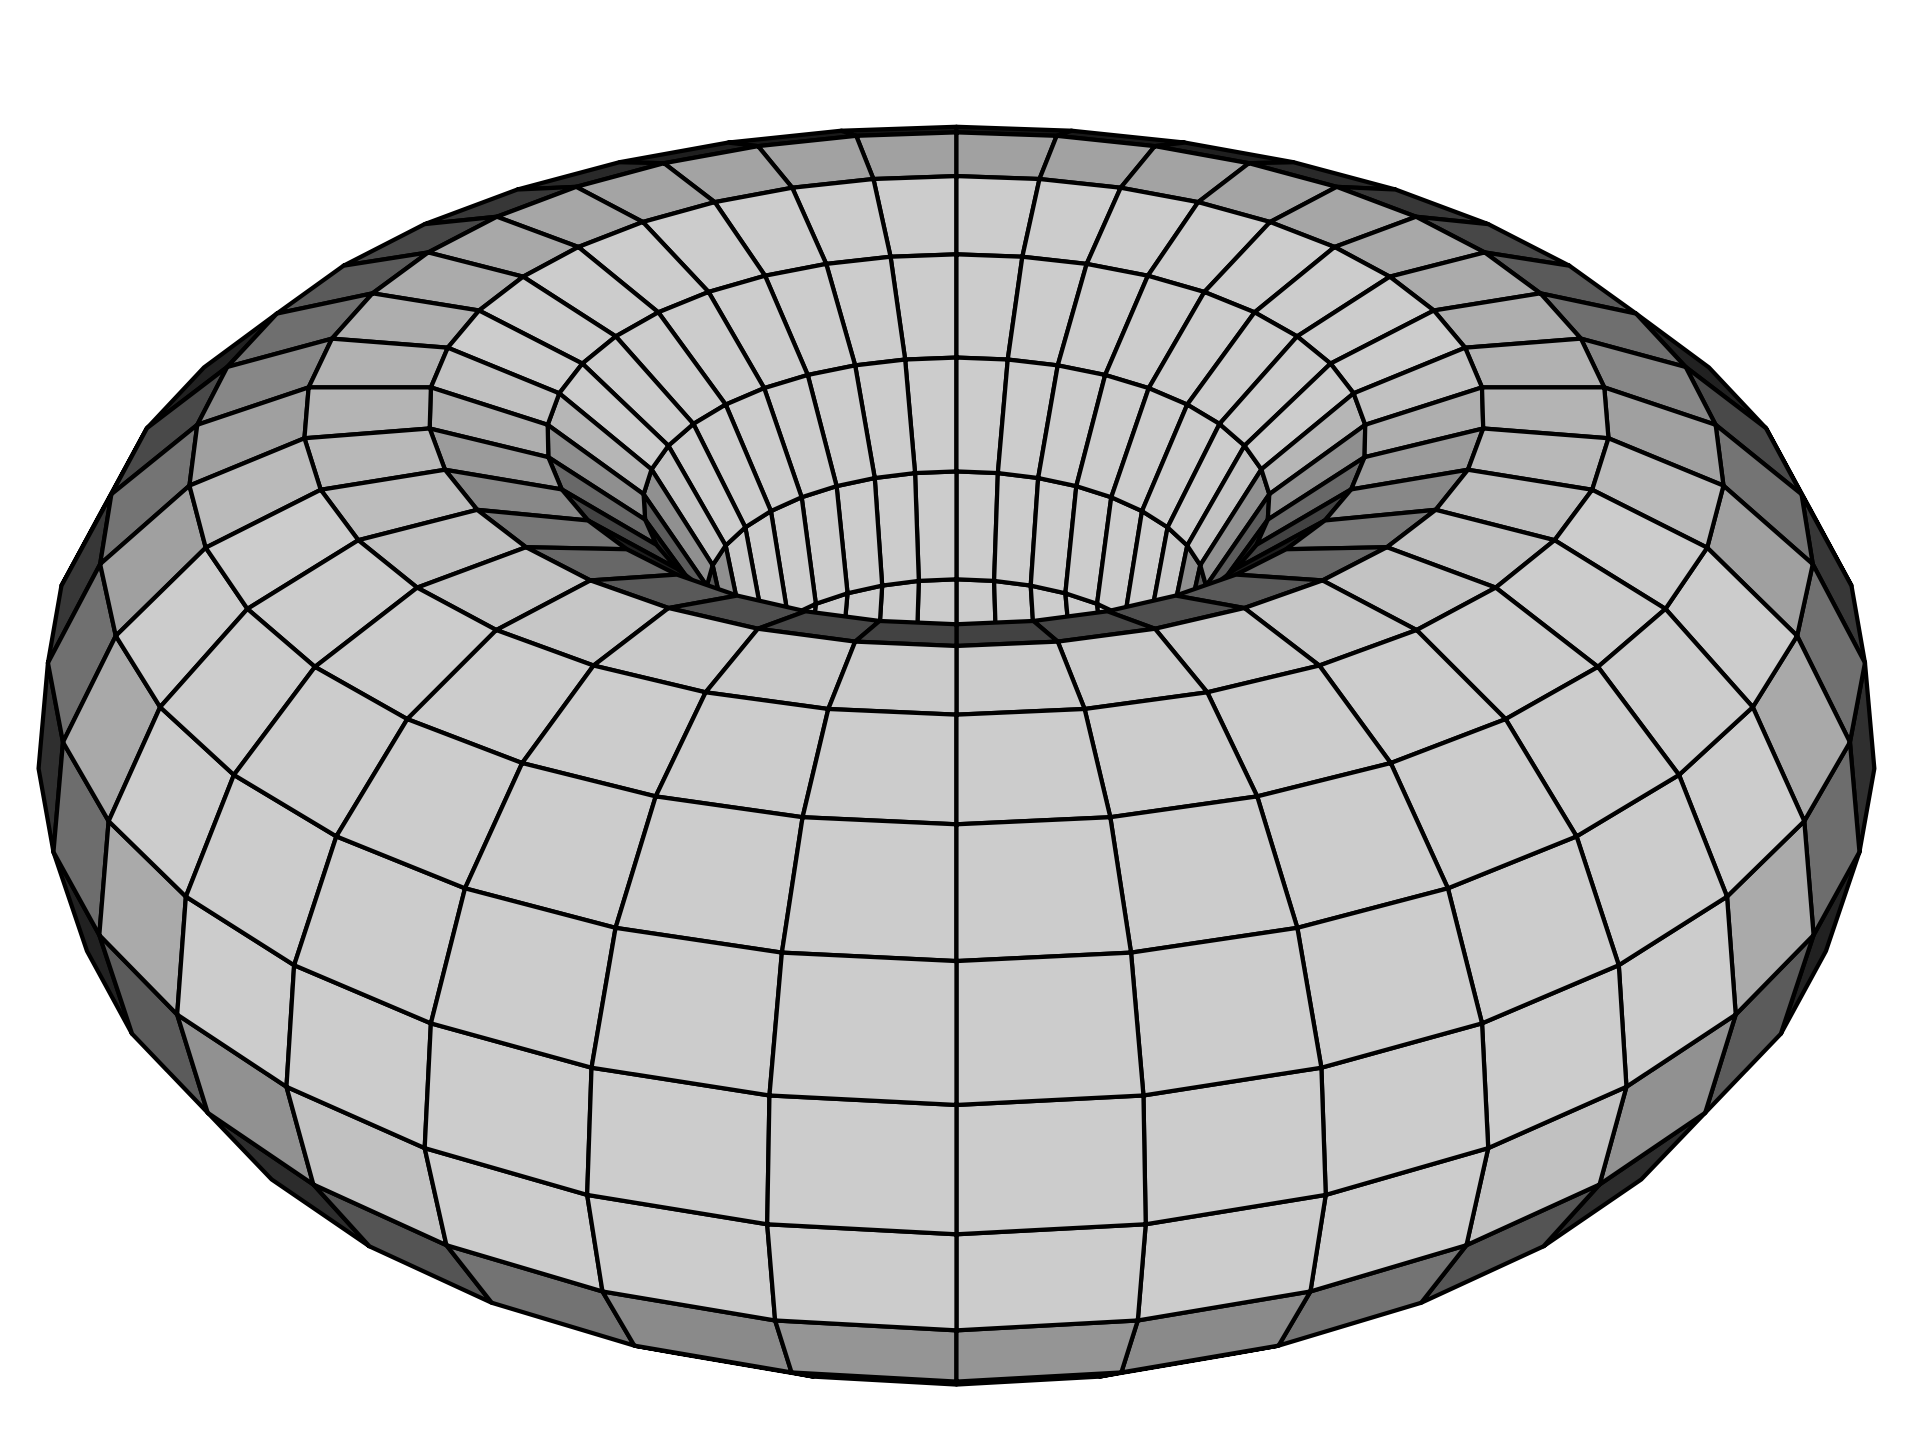
\includegraphics[width=0.3\textwidth]{./torus.png}};


\node at (1.1-5,8.6-10) [draw=none, rectangle, fill=darkblue,rotate=0] (g1) {};

\node at (1.1-5, 8.2-10) [draw=none, rectangle, fill=gold,rotate=0] (g2) {};

\node at (2.2-5,8.6-10) [draw=none, rectangle, fill=none,rotate=0] (g1) {\sf \small \emph{E. coli} OP50};

\node at (3.1-5,8.2-10) [draw=none, rectangle, fill=none, rotate=0] (g1) {\sf \small \emph{Novosphingobium} sp. L76};

% %labels
% \draw (-4.2, 10.4) node{{\footnotesize\sf\textbf{P}}};

% \draw (-5, 12) node{{\Huge\sf\textbf{b}}};

% \draw (-6.5, 0) node{{\Huge\sf\textbf{c}}};

% \draw (-6.5, -3.5) node{{\Huge\sf\textbf{d}}};



\end{tikzpicture}


\end{document}